In this chapter we present some background related to analytic in the domain of soccer. We look at different types of analysis out there. This spans from pre-match to post-match. Then we go into how data is gathered and presented. For gathering of data there are two main approaches: manually often by humans annotating video feeds, and automatic capturing often by installing receivers and having players wear physical sensors for tracking.

\section{Types of analysis}

In soccer there are several phases where you use analytic to help you gain insight. In this section we will look at the typical use cases of analytic. Not only soccer teams use analytics, but also broadcasting companies and fans widely use statistics to build up under their arguments.

\subsection{Pre-match}

Pre-match you use analytic to find weaknesses and strengths in the opponent team, on an individually level or as a team. You look at your team matched up against your opponent. A typical situation is that the manager gets a video summary of the opponent highlighting the opponent’s strengths and weaknesses. The coaching staff may use tools like Interplay to gather information and create the video summary. Other software like Prozone\footnote{http://www.prozonesports.com/index.html} can also likely be used to break down the opponents offensive and defensive play. A deeper introduction to Prozoen is given in section \ref{sec:prozone}

Typically in TV you have pundits bringing you analytic of key battles during the build up to the game. A typical thing is to look at battles like wingers versus backs, midfield clashes or striker versus central defenders. The battles are often illustrated with statistics or with video clips highlighting aspects of both players game that will be decisive. 

Fans are analyzing the game all the time. Except from TV they get exposed to analytic via social media. Opta\footnote{http://www.optasports.com/} is company that has taken full advantage of social medias. Figure \ref{fig:optastats} is a screenshot of a tweet from one of the many accounts Opta control. 

\begin{figure}[ht!]
\centering
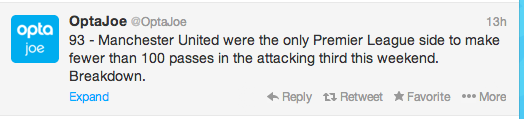
\includegraphics[width=1\textwidth]{images/general/optastats.png}
\caption{A typical tweet from one of Opta's Twitter account}
\label{fig:optastats}
\end{figure}

\subsubsection{In match}

During match the coaching staff continuously analyze the match and make adjustment. The players make all the decisions in the end, but the coach is the boss and sets the style of play. An adjustment to the teams formation can potentially be the tipping point that wins you the game.

Tromsø IL uses a system Muithu \cite{muithu} that lets you annotate sequences of a game with entity's like player and comment. This information will then be time synchronized with the video feed. Later, like in at half time or even in the game, you can search on entity's to get the corresponding video feed. It can be anything that has been previous tagged like a player involvement to a team move that was executed perfectly. 

Using systems like \ac{ZXY}\footnote{http://www.zxy.no} or MiCoach \cite{bigdata:majorleague} you can get real time information about a players performance during the match. Rather than assuming that a player is tiring you can get information metrics that tells you this. You get evidence that the player in fact is fatigued. In soccer you only have 3 substitutions. Making the right ones is crucial in an even match or to avoid injuries.

Using data gathered from sports data company's like Opta you can get statistics live during the game. It is popular in TV to show statistics like ball possession percent, how far players have run or the number of passes played and so on. As mentioned earlier Opta posts many of their statistics to their social media accounts.

\subsection{Post match}

During the post match the coach team goes through the game to evaluate the team performance. This is valuable as you get concrete clips about good and bad involvements on team or player level. You can highlight situations in the match to help players better understand tactical aspects. Interplay Sports\footnote{ http://www.interplay-sports.com/} is a system used today at Alfheim for this purpose. It is used for analysis of matches in a post-match scenario where you can tag situations in the video. 

\section{Capturing of data}
\subsection{Opta}

Opta, one of the big players in the field of sport analytic uses manual input to create their data repository \cite{dailymailOnStatistics}. They have editorial teams across the world that captures data manually for the most popular soccer leagues and other sports. For example to capture statistics for a single match they have 3 humans annotating. The data is captured via an application specifically created for the purpose of capturing data as quick and easily as possible. The editorial teams of Opta need to be able to identify a player in a very short time to be able to keep up with the pace of the game. 

Opta capture all types of actions like passes, type of pass, attacks, and interceptions to mention a few. For each action they log, they add a series of description tags like pitch coordinate, timestamp, which player and team. For every single pass they add descriptors if it was a through ball, normal ball or even as detailed a headed flick on from a long ball. For shots they register the foot it was kicked with, if it was a volley and so on. All this is done while the match is playing. About 1600 individual events are recorded in a standard match. This gives them a very rich database of events and a range of possible queries to run. 

\begin{lstlisting}
<Event id="290575408" event_id="5" type_id="1" 
player_id="20856" team_id="810"  x="44.6"y="61.1">
   <Q id="1774596260" qualifier_id="141" value="91.6"/>
   <Q id="1429253465" qualifier_id="140" value="49.9"/>
   <Q id="1084400575" qualifier_id="56" value="Back"/>
</Event>
\end{lstlisting}

Above is an example of an event extracted from the Opta database (stripped down). The event has a series of qualifiers describing it. We see that x and y coordinates for the pass and the outcome of the event are registered. In this example the event is a pass from [44.6, 61.1] to [91.6, 49.9] in Opta’s co-ordination system.

\subsection{Prozone}
\label{sec:prozone}
Prozone is a video-based system that tries to track players in team sports \cite{Prozone:indepth}. Their data capture system incorporates 8-12 cameras, which is strategically positioned throughout the stadium to cover 100 percent of the ground, but with some redundancy in case of a faulty component. They also incorporate the TV-camera feed, which always follows the ball. All cameras are hooked into one server and uploaded at the end of the game before sent to undertake the tracking process. When the system is installed it required some setup before it is operational; the pitch size needs to be incorporated into the system and cameras calibrated. Figure \ref{fig:prozonecam} shows the camera location in a soccer stadium.

\begin{figure}[ht!]
\centering
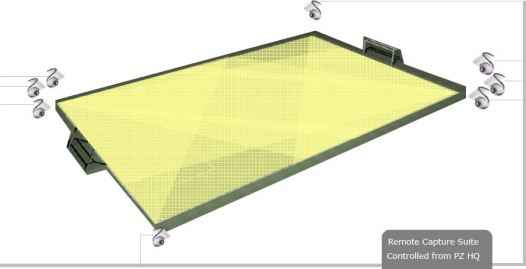
\includegraphics[width=1\textwidth]{images/general/prozonecam.png}
\caption{The Prozone camera system illustrated. Taken from Prozonesports.com}
\label{fig:prozonecam}
\end{figure}

The coding tracking process of the player's movement and actions is a sort of manual process at present time. First each camera feed goes through each own tracking process determining image co-ordinates and continuous trajectories for each player. The output from all the cameras is then combined into one dataset. Going into the algorithm for this is out of the scope of this project. In the final stage the manual work comes into the loop. There has to be a quality control group of operators dedicated for post processing the game. First, the operators have to map the player’s identity with their corresponding start location. The operators will then follow the video feed checking that the identification of all players remains constant during the match. The tracking process may run into problems when two players collide or have any other physical contact as it becomes unclear who is who. To map video image co-ordinates to pitch co-ordinates Prozone uses computer vision homography calibration process.

The whole manual operation by the operators is done in an own software that helps you minimize the amount of manual work for the operators. The software follows rules created by basic machine learning algorithms to validate and verify the input. A simple example would be if the ball goes out of play the system would know that the next event would be a throw in, corner kick or goal kick.

Prozone claims to be able to track every movement of every player on the pitch with a resolution of 10th of a second. This without using any physical equipment on the players. Di Salvo et al. \cite{Prozone:validation} conducted an empirical evaluation of deployed Prozone systems at Old Trafford in Manchester and Reebook Stadium in Bolton, and concluded that the video camera deployment gives an accurate and valid motion analysis. The data after a match is available through Prozone analysis software. 

\subsection{Automatic capturing}

A system that uses sensors is \ac{ZXY} . The system is used by premier league soccer teams in Norway, including \ac{TIL} and Rosenborg BK. Data captured is stored in a Sybase database with each match requiring about 500-700MB storage. The players have to wear a belt around their waist for the system to be able to track their movements. The ZXY system is able to track the player’s movement very detailed with an accuracy of 0.5m. It has a resolution of 20 samples per second. 

The technology behind it relies on a radio-based signaling substrate to provide real-time high-precision positional tracking, also including acceleration and heart rate \cite{PTW}. An installation of receivers is required for the system to work. The home arena for \ac{TIL}, Alfheim, is currently equipped with 10 receivers. A receiver tracks a specific area of the soccer field and combined they cover the whole pitch with some redundancy areas. The communication from the belt to the receivers goes on a 2.45-5.2 G Hz frequency radio signal. To compute the positional data the stationary radio receiver uses an advance vector based processing of the received radio signal. The data is aggregated and stored into a relational database. Including the positions of the players ZXY also gives you the step frequency, speed and direction.

\begin{figure}[ht!]
\centering
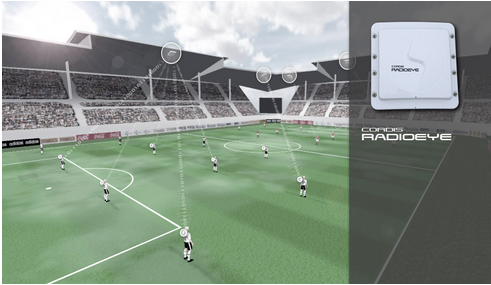
\includegraphics[width=1\textwidth]{images/general/zxyoverview.png}
\caption{Overview of the ZXY system with receivers placed at the stadium and players wearing sensors. Image from zxy.no}
\label{fig:zxycam}
\end{figure}

\subsection{Wrap up}
The main problem with tracking systems that uses physical sensors is that usually only one of the teams wears the sensors. This limits the functionality of the system as an opponent analysis system. You only get data for one team and if you have installed it at your stadium it captures only half of the matches. 

On the other hand you have the manually systems that require human annotation of matches. These systems have the advantage of being able to track both teams. As they rely on human annotation of some degree they get more rich data as well, but requires strict rules of the semantics of the metadata. There has to be some form of quality control of the data captured to ensure correctness. 

\section{Presenting data}

This section gives a short overview of how some systems presents information.

\subsection{Prozone}

Prozone comes with several systems to illustrate data gathered. The most relevant for this project is the opposition analysis system\footnote{http://www.prozonesports.com/service-opposition-analysis.html}, but also several other tools Prozone delivers can be used in opponent analytic. The tools includes features like 2D animation, single player analysis, team analysis, pressing analysis, player tempo, passing movements, receiving the ball and player events. Figure \ref{fig:prozone} shows some of this features.

\begin{figure}[ht!]
\centering
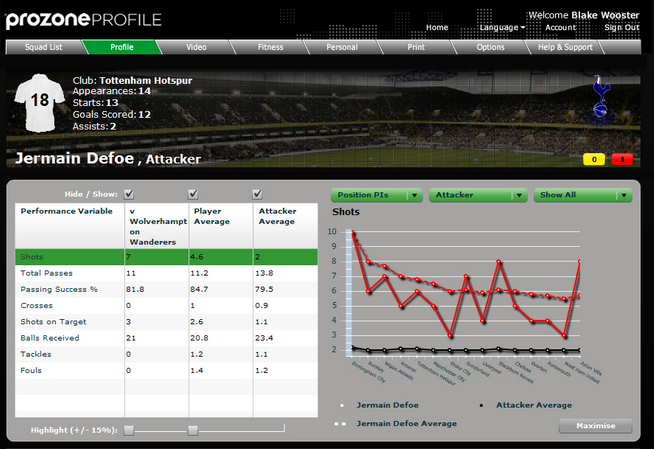
\includegraphics[width=1\textwidth]{images/general/prozonestats.png}
\caption{The Prozone software - individual player analysis gives you statistics of performance over time. Image from prozonesports.com}
\label{fig:prozone}
\end{figure}

On individual level you can get basic statistics like shots, total passes, passing success, crosses, shots on target, balls received, tackles and fouls. 
You can also retrieve all sprints for a player. This could help you prevent injuries. Players in certain areas of the field have more intensive sprints when they first are involved and thus are more vulnerable to injuries. Knowing the actual physical load on players the coaching staff can regulate the training intensity and amount of time on each exercise for each individual.

\subsection{ZXY Sport Tracking System}
ZXY provides you with a 3D graphic interface showed in figure \ref{fig:zxysoftware}. This interface lets you see the player’s action in real time by reading the data stream to reproduce actions by players. The data is streamed in real time into the database as the match goes on. While watching you can produce timestamps of different events and produce manual input, which is time synchronized with the automatic data. Naturally, you can build your own software on top of the Sybase database. \ac{TIL} in collaboration with University of Troms{\o} has made several systems to complement the ZXY software; Muithu\cite{muithu} and Bagadus\cite{Saegrov2012}.

\begin{figure}[ht!]
\centering
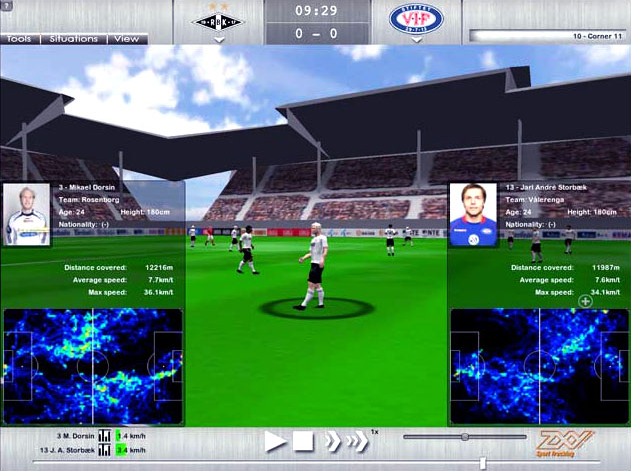
\includegraphics[width=1\textwidth]{images/general/zxysoftware.png}
\caption{The ZXY software - tracking of players gives you information of distance covered, average speed and max speed. You also get a heat map of the player’s movement on the field. Image from zxy.no}
\label{fig:zxysoftware}
\end{figure}

\subsection{FourFourTwo}

FourFourTwo is a monthly magazine about football. They also have a webpage which they update daily. Particular, they focus on match analytic with Opta providing them data. All the analyses posted on their web page are created by using their own developed application Stats Zone. The application is available for everyone and it’s a popular among blogs writing about soccer analytic. Figure \ref{fig:fourfourtwo} shows a typical graphical illustration done with the Stats Zone application highlighting passes in to attacking third of the pitch. 

\begin{figure}[ht!]
\centering
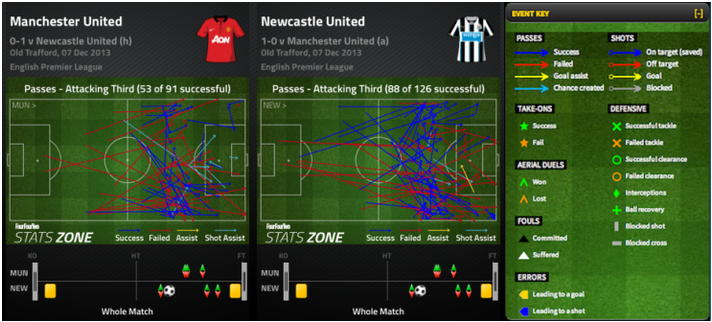
\includegraphics[width=1\textwidth]{images/general/fourfourtwo.png}
\caption{Illustration of all passes in to attacking third in the match Manchester United vs Newcastle United. Taken from fourfourtwo.com}
\label{fig:fourfourtwo}
\end{figure}



